\documentclass[10pt]{article}
\usepackage{float}
\RequirePackage{eso-pic}
\usepackage{caption}
\captionsetup[table]{labelformat=empty}



\usepackage{geometry}
\geometry{
a4paper,
left=11mm,
right=14mm,
top=37mm,
bottom=14mm,
}



\usepackage{colortbl}
\usepackage{fontspec}
\setmainfont[Ligatures=TeX]{Calibri}



\newcommand\BackgroundPic{%
\put(0,0){%
\parbox[b][\paperheight]{\paperwidth}{%
\vfill
\centering
\includegraphics{MBIE_generic_background.pdf}%
\vfill
}}}



\begin{document}
\thispagestyle{empty}
\AddToShipoutPicture{\BackgroundPic}
\section*{Key Export Statistics\footnotemark - Avocados\footnotemark }
Published on April 07, 2016. \par
\small{\noindent{\textit{Monthly data from January 2000 to November 2015.}}}
\begin{table}[ht]
\centering
{\scriptsize
\begin{tabular}[t]{p{1.8cm}>{\hfill}p{1.4cm}>{\hfill}p{1.4cm}>{\hfill}p{1.6cm}>{\hfill}p{1.9cm}>{\hfill}p{2cm}>{\hfill}p{1.9cm}>{\hfill}p{1.5cm}}
 \textbf{Country} & \textbf{Yearly Qty} & \textbf{Yearly Value} & \textbf{Yearly Price} & \textbf{3Year CAGR(Qty)} & \textbf{3Year CAGR(Value)} & \textbf{3Year CAGR(Price)} & \textbf{Price Elasticity} \\
\hline
Australia & 15,842 & 83.2 & \$5.3 & 18.8\% & 20.8\% & 1.6\% & 11.5 \\  
Thailand & 561 & 3.8 & \$6.9 & 224.8\% & 285\% & 18.5\% & 12.1 \\  
Singapore & 742 & 3.6 & \$4.8 & 12.8\% & 19.6\% & 6\% & 2.1 \\  
Japan & 701 & 2.5 & \$3.5 & -3.4\% & -1.2\% & 2.2\% & -1.5 \\  
South Korea & 364 & 2.4 & \$6.5 & 21.6\% & 44.1\% & 18.5\% & 1.2 \\  
Malaysia & 106 & 0.5 & \$5.0 & 18.2\% & 30.4\% & 10.3\% & 1.8 \\  
Other & 128 & 0.9 & \$6.8 & 26.4\% & 42.9\% & 13.1\% & 2.0 \\  
Total & 18,443 & 96.9 & \$5.3 & 18.5\% & 22.1\% & 3\% & 6.2 \\  
\hline
\end{tabular}
}
\caption{\scriptsize Top 6 Avocados Markets for year ending November - 2015: Quantity('000 kg) Value(NZ\$Mill), Price and their last 3-Year Growth Rates}
\end{table}


\vspace{-0.7cm}



   \begin{figure}[H]
   \centering
    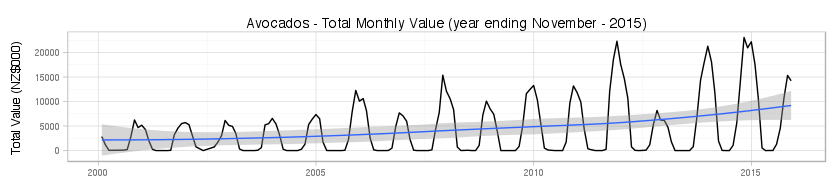
\includegraphics[scale=0.5]{../graphs/monthly_value/avocados_monthly_value.png} \
    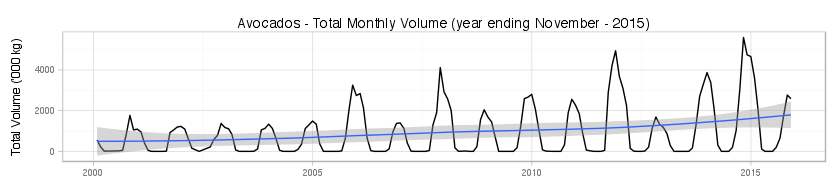
\includegraphics[scale=0.5]{../graphs/monthly_volume/avocados_monthly_volume.png} \
    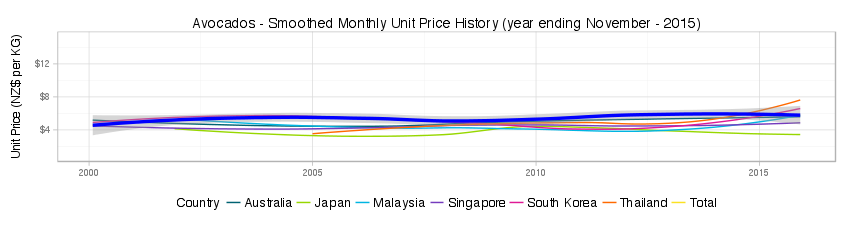
\includegraphics[scale=0.5]{../graphs/smoothed_price/avocados_smoothed_price.png} \
    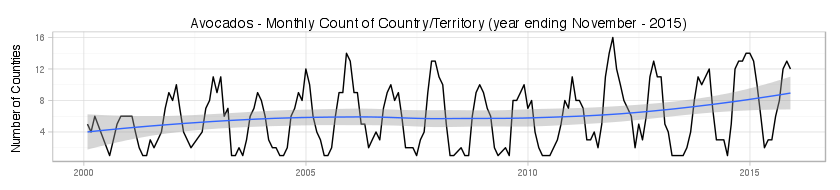
\includegraphics[scale=0.5]{../graphs/monthly_number_countries/avocados_monthly_count.png} \
    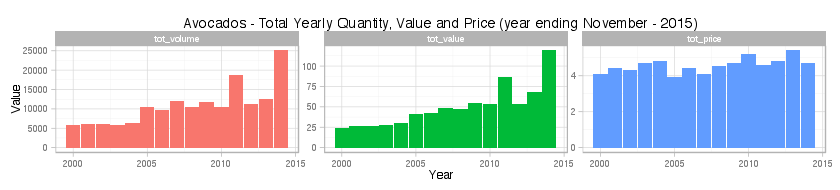
\includegraphics[scale=0.5]{../graphs/yearly_summary/avocados_yearly_summary.png} \
   \end{figure}



\footnotetext[1]{Source: Statistics New Zealand - Overseas Merchandise Trade}
\footnotetext[2]{Harmonised System Codes for Avocados starting with: 080440.}
\end{document}
